\chapter{Double deep Q-learning Solution}

We will start this chapter by describing deep Q-learning and then present it's result.

\textbf{Deep reinforcement learning} is the combination of Reinforcement learning and
deep learning. \textbf{Q-learning} is one of the \textbf{off-policy} learning that trains the agent
and tells what is the optimal action to take in each state. This approach can be used
when the number of state-action pairs are limited enough to store there q-value in
the memory. Even if we are able to store q-value of each state-action pair, it is
highly inefficient because the agent need to visit each state-action pair for
reasonable number of times to learn their q-values. Since the total state-action pair
can be very high for real life problems , better approach would be to use the
\textbf{function approximator\cite{BOOK:1}} that approximates the q-value once the state and action are
given as the input. Since neural networks can be used as the function
approximators, so here is the point where deep learning and reinforcement
learning are combined to train the agents to perform in an environment.
In this report, we will be working on DDQN (double deep Q-learning), although there are
whole different class of policy gradient approaches.

\section {Algorithm}

Bellman equation describing the optimal action-value function, $Q^*(s,a)$ is given by,
$$Q^*(s,a) = \mathop{\mathbb{E}}_{s' \sim P}[r(s,a) + \gamma \mathop{\max}_{a'}Q^*(s',a') ]$$

where $s' \sim P$ is shorthand for saying that the next state, s' is sampled by the environment from a 
distribution $P(.|s,a)$

\vspace{\baselineskip}
This Bellman equation is the starting point for learning an approximator to $Q^*(s,a)$. 
Suppose the approximator is a neural network $Q_{\phi}(s,a)$, with parameters $\phi$, 
and that we have collected a set ${\mathcal D}$ of transitions $(s,a,r,s',d)$ (where $d$ 
indicates whether state $s'$ is terminal). We can set up a \textbf{mean-squared Bellman error (MSBE)} function,
 which tells us roughly how closely $Q_{\phi}$ comes to satisfying the Bellman equation:

$$ L (\phi , \mathcal D) = \mathop{\mathbb{E}}_{(s,a,r,s',d) \sim \mathcal D} \left[ \left(Q_{\phi}(s,a) - (r + \gamma(1 - d)\mathop{\max}_{a'} Q_{\phi}(s',a') )\right) ^2 \right] $$ 

When $d==$True , which is to say, when $s'$ is a terminal state—the Q-function should show that the 
agent gets no additional rewards after the current state. 

\vspace{\baselineskip}
Q-learning algorithms for function approximators, such as DQN(and all its variants\cite{ARTICLE:5}, \cite{ARTICLE:6}) are largely based
on minimizing this MSBE loss function. There are two main tricks employed.

\vspace{2.0cm}
\textbf{Trick One : Replay Buffers}
All standard algorithms for training a deep neural network to 
approximate $Q^*(s,a)$ make use of an experience replay buffer. 
This is the set ${\mathcal D}$ of previous experiences. 
In order for the algorithm to have stable behavior, the replay buffer should be large enough to 
contain a wide range of experiences, but it may not always be good to keep everything. 
If you only use the very-most recent data, you will overfit to that and things will break; 
if you use too much experience, you may slow down your learning. We are using a \textbf{buffer replay of size $10^5$}.

\vspace{\baselineskip}
\textbf{Trick Two : Target Networks}. Q-learning algorithms make use of target networks. The term 
$$ r + \gamma(1-d)\mathop{\max}_{a'}Q_{\phi}(s',a')$$

is called the \textbf{target}, because when we minimize the MSBE loss,
 we are trying to make the Q-function be more like this target. 
 Problematically, the target depends on the same parameters we are trying to train: $\phi$. 
 This makes MSBE minimization unstable. The solution is to use a set of parameters which comes close
  to $\phi$, but with a time delay - that is to say, a second network, called the \textbf{target network},
   which lags the first. The parameters of the target network are denoted $\phi_{\text{targ}}$.

\vspace{\baselineskip}
The target network is just copied from the main network every some fixed number of states. In our work,
the target network is updated once per main network update by polyak averaging:
$$ \phi_{\text{targ}} \leftarrow \rho \phi_{\text{targ}} + (1 - \rho)\phi$$
where $\rho$ is a hyperparameter between 0 and 1 (usually close to 1).
\vspace{10cm}
\subsection{Pseudocode}

\begin{algorithm}[h]
    \caption{ Double Deep Q-learning \cite{ARTICLE:5} }
    \begin{algorithmic}
    \State Initialize primary network $Q_{\phi}$ , target network $Q_{\phi_{\text{targ}}}$ , replay buffer  $\mathcal D$,  $\rho \ll 1$
    \State \textbf{for} each Iteration \textbf{do}:
    \State \;\;\;\;\;\;\textbf{for} each environment step \textbf{do}: 
    \State \;\;\;\;\;\;\;\;\;\;\;\;Observe state s and select $a \sim \pi(a,s)$
    \State \;\;\;\;\;\;\;\;\;\;\;\;Execute a in the environment
    \State \;\;\;\;\;\;\;\;\;\;\;\;Observe next state $s'$ , reward r, and done signal d to indicate wether $s'$ is terminal
    \State \;\;\;\;\;\;\;\;\;\;\;\;Store $(s,a,r,s',d)$ in replay buffer $\mathcal D$
    \State \;\;\;\;\;\;\;\;\;\;\;\;If $s'$  is terminal, reset environment state.    
    \State \;\;\;\;\;\;\textbf{for} each update step \textbf{do}
    \State \;\;\;\;\;\;\;\;\;\;\;\;Randomly sample a batch of transitions, $B = {(s,a,r,s',d)}$ from $\mathcal D$
    \State \;\;\;\;\;\;\;\;\;\;\;\;Compute targets
    \State $$Q^*(s,a) \approx r + \gamma (1-d) Q_{\phi}(s' , \mathop{\text{argmax} }_{a'} Q_{\phi_{\text{targ}}}(s',a') )$$
    \State \;\;\;\;\;\;\;\;\;\;\;\; Update Q-function by one step of gradient descent using
    \State $$\nabla_{\phi} \frac {1}{|B|} \sum_{(s,a,r,s',d) \in B} (Q_{\phi}(s,a) - Q^*(s,a)  )^2  $$    
    \State \;\;\;\;\;\;\;\;\;\;\;\; Update target network with
    \State $$ \phi_{\text{targ}} \leftarrow \rho \phi_{\text{targ}} + (1 - \rho)\phi$$
    \end{algorithmic}
    \end{algorithm}
    
\section {Results}
We used DDQN algorithm on flatland environment using tree observation. Although,
it is reasonable to assume that an observation of the full environment is beneficiary for good global solutions. it used to work 
only on small toy examples (even these are hard to train). However, we run into problems when scalability and flexibility
 become an important factor. Already on small toy examples we could show that flexibility quickly becomes an issue
  when the problem instances differ too much. When scaling the problem instances the decision performance of the algorithm 
  diminishes and re-training becomes necessary. On real life instances, we do not believe that a global observation is suited for this 
  problem. So we used DDQN algorithm only on using tree observation.

\vspace{\baselineskip}
In order to use the tree observation, we flat out the tree creating a linear vector whose size depends on tree depth and 
number of features in each node. Since increasing the tree depth increases the size of vector exponentially,
using larger tree depth (of the order of 5,6) can have vector of size of order ($10^4$ to $10^5$).
 In our case we worked on tree depth 2 and 3. Also, we include malfunction (making the problem much harder) in the agents, as this will add 
 stochasticity into the system and helps in better training instance.


 \subsection{Single agent}
 When trained on environment having single agent, the results are very good. This is because, since there is only one 
 agent, the whole environment is stationary with respect to the agent.During the course of training over 2000 episodes on real life example,
 as the training proceeds agent is able to reach the target within time bound ((3*(env.height + env.width)). Moreover, 
 agent is able to find the shortest path as evident from the figure 7.2. Notice that the underlying railway network and
 the schedule of trains (starting position and target) keeps on changing during the course of training. Only certaing specifications
 like number of cities, number of parallel tracks connecting city, number of agents, malfunction rate etc. is fixed.

 \begin{figure}[h]
    \centering
    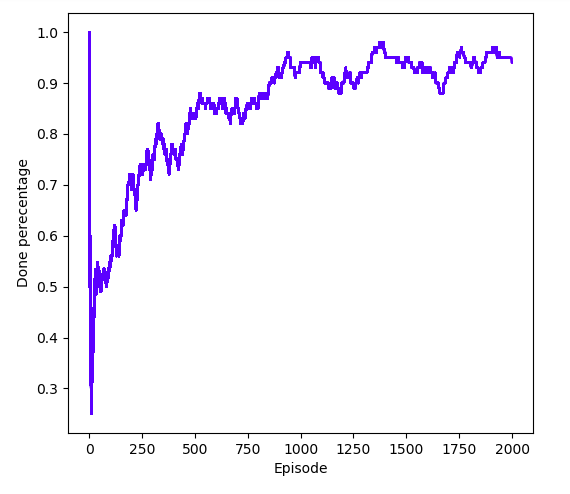
\includegraphics[width=0.5\textwidth]{single_agent_tree_observation_depth2}
    \caption{ Percentage of agents able to complete journey. Single agent, 5 cities, with 2 rails 
    connecting each city with tree depth 2 }
    \label{result10}
\end{figure}

\begin{figure}[h]
    \centering
    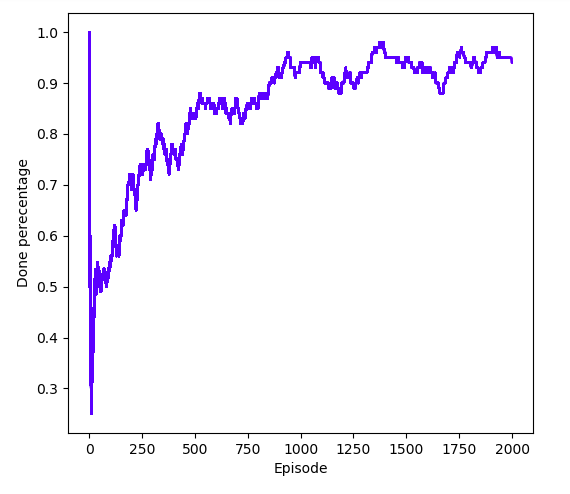
\includegraphics[width=0.5\textwidth]{single_agent_tree_observation_depth2}
    \caption{ Percentage of agents able to complete journey. Single agent, 5 cities, with 2 rails 
    connecting each city with tree depth 2 }
    \label{result10}
\end{figure}

\subsection{Multiple Agent}
The Q-learning algorithm assumes that the environment is stationary for the convergence property. Since in case of multiagent 
environment, environment is non-stationary from the point of view of single agent, so convergence is not guaranteed. 
Although, it is possible that the agent learns what is best possible action for itself given a particular observation but there 
is no way, agent can cooperate perfectly. 

\begin{figure}[H]
    \centering
    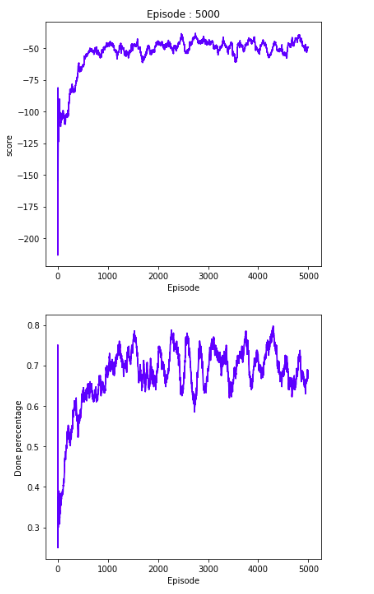
\includegraphics[width=0.5\textwidth]{agent4_city_3_multi}
    \caption{Result of training over real life railway network with 4 agents, 3 cities and tree depth 2 for 5000 episodes. 
        (A) Score of agent, this shows the average reward of agents as the training progresses. 
        (B) Percentage of agents able to complete journey as the training progresses. }
    \label{result10}
\end{figure}

The result shows that, 80\% of the agents are able to complete there journey using short paths when railway network have 4 agents, 3 cities. 
So the results are good when the number of agents is small (in this case 4).

\begin{figure}[H]
    \centering
    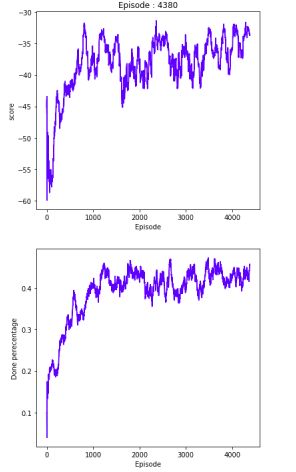
\includegraphics[width=0.5\textwidth]{agent10_city3_multi}
    \caption{Result of training over real life railway network with 10 agents, 3 cities and tree depth 2. 
        (A) Score of agent, this shows the average reward of agents as the training progresses. 
        (B) Percentage of agents able to complete journey as the training progresses. }
    \label{result10}
\end{figure}

So as the number of agents increases to 10, with everything else same, only 40\% of the agents are able to complete there
journey. The results are even worse, when the number of agents increases more.

\section{Alternate RL algorithms}
Q-learning algorithm is designed having the assumption that the environment is stationary with respect to the 
agent. But in case of multiagent environment, environmnent is non stationary with respect to the agent, violating Markov assumptions required for 
convergence of Q-learning. There are RL algorithms for multiagent environment. One of the most effective is 
\textbf{Multi-Agent Actor-Critic for Mixed
Cooperative-Competitive Environments (MADDPG)\cite{ARTICLE:7}} based on actor critic based approach for single agent. 
In the next chapter, we will solve the same problem using cooperative path finding. 